
\subsection*{Lösungen zu den Kapitel~\ref{kapitel:GraphenInCombo}: \emph{Kombinatorikaufgaben mit Graphentheorie lösen}}

\begin{proof}
	Wir betrachten den Graphen $G$, dessen Knoten die Orte und dessen Kanten die Feldwege sind. Wir dürfen ohne Einschränkung annehmen, dass $G$ zusammenhängend ist (ansonsten führen wir das folgende Argument in jeder Zusammenhangskomponente durch). Dann hat jeder Knoten von $G$ Grad $3$. Weil die Anzahl der Knoten ungeraden Grades stets gerade ist, muss $G$ gerade viele Knoten haben. Wir teilen die Knoten von $G$ beliebig in Paare auf und fügen für jedes Paar eine Kante hinzu (wenn dadurch parallele Kanten entstehen, ist das kein Problem). Nun hat jeder Knoten Grad $4$, also gibt es nach dem Satz von Euler-Hierholzer einen geschlossenen Weg, der jede Kante genau einmal durchläuft. Entlang dieses Weges färben wir die Kanten abwechselnd rot und grün. Dann hat jeder Knoten zwei rote und zwei grüne ausgehende Kanten. Das gilt insbesondere auch für den ersten (und letzten) Knoten des Weges, denn nach dem Handschlagslemma ist $4\abs{V}=\sum_{v\in V}d(v)=2\abs{E}$, also ist $\abs{E}$ gerade. Nun entfernen wir die hinzugefügten Kanten wieder. Dann hat jeder Knoten immer noch mindestens eine rote und mindestens eine grüne ausgehende Kante. Wenn wir alle roten Kanten zu Radwegen ausbauen, haben wir also die Aufgabe gelöst.
\end{proof}

\begin{proof}[Lösung zu Aufgabe~\ref{aufgabe:50Laender}]
	Für~\ref{teilaufgabe:50} betrachten wir den Graphen $G$, dessen Knoten $v_1,v_2,\dotsc,v_{100}$ die 100 Leute sind. Je zwei Leute aus einem Land verbinden wir mit einer Kante; diese Kanten nennen wir \emph{Länderkanten}. Außerdem verbinden wir $v_1$ mit $v_2$, $v_3$ mit $v_4$, \ldots, $v_{99}$ mit $v_{100}$; diese Kanten nennen wir \emph{Nachbarskanten}. Wenn dabei parallele Kanten entstanden sind, ist das nicht schlimm. Jeder Knoten von $G$ hat Grad $2$, also ist $G$ eine disjunkte Vereinigung von Kreisen. In jedem Kreis wechseln sich außerdem Länder- und Nachbarskanten ab, also hat jeder Kreis gerade Länge. Nun durchlaufen wir jeden Kreis und färben die Knoten abwechselnd rot und grün. Indem wir alle roten Knoten die eine Gruppe bilden lassen und alle grünen Knoten die andere, haben wir die Aufgabe gelöst.
	
	Für~\ref{teilaufgabe:25} teilen wir jedes der 25 Länder temporär in zwei Teile auf, sodass aus jedem Teil genau zwei Leute kommen. Wir teilen die 100 Leute zunächst wie in~\ref{teilaufgabe:50} in zwei Gruppen $G_1$ und $G_2$ auf. In $G_1$ verbinden wir je zwei Leute aus einem Land mit einer Kante. Außerdem verbinden wir alle Paare von Leuten, die vorher im Kreis nebeneinander standen. Diese Kanten nennen wir wie vorher \emph{Länder-} und \emph{Nachbarskanten}. Nach Konstruktion geht von jedem Knoten von $G_1$ eine Länderkante aus. Da es in $G_1$ keine drei Leute gibt, die vorher im Kreis nebeneinander standen, geht von jedem Knoten maximal eine Nachbarskante aus. Die Knoten, von denen noch keine Nachbarskante ausgeht, teilen wir beliebig in Paare auf und verbinden jedes Paar. Etwaige parallele Kanten sind uns dabei wieder egal. Analog zu~\ref{teilaufgabe:50} zerfällt $G_1$ in Kreise gerader Länge, in denen sich Länder- und Nachbarskanten abwechseln. Indem wir die Kreise wieder alternierend färben, haben wir $G_1$ in zwei Gruppen mit den gewünschten Eigenschaften aufgeteilt. Analog verfahren wir mit $G_2$.
\end{proof}

\begin{proof}[Lösung zu Aufgabe~\ref{aufgabe:Kartenspiel}]
	Wir betrachten den gerichteten Graphen $G$, dessen Knoten die möglichen Spielsituationen sind (eine Spielsituation wird stets eindeutig durch die beiden Kartenstapel beschrieben). Zwischen zwei Spielsituationen $s_1$ und $s_2$ ziehen wir genau dann eine gerichtete Kante $s_1s_2$, wenn $s_1$ im nächsten Zug zu $s_2$ führen kann. Fast jeder Knoten hat dann Ausgangsgrad $2$, denn in jedem Zug gibt es zwei Möglichkeiten, in welcher Reihenfolge die Gewinnerin ihre beiden gewonnenen Karten unter ihren Stapel legt. Die einzigen Knoten, die nicht Ausgangsgrad $2$ haben, sind die Spielsituationen, in denen eine Mathematikerin keine Karten mehr hat. In diesem Fall ist das Spiel endlich vorbei und der Ausgangsgrad ist $0$.
	
	Andererseits hat jeder Knoten höchstens Eingangsgrad $2$. Denn für jede Spielsituation gibt es höchstens zwei Möglichkeiten, welche Mathematikerin den letzten Zug gewonnen hat (falls eine Mathematikerin maximal zwei Karten in ihrem Stapel hat, gibt es sogar nur eine Möglichkeit, denn sonst wäre das Spiel schon vorbei gewesen). Für jede Möglichkeit ist die vorherige Verteilung durch die beiden untersten Karten im Stapel der Gewinnerin eindeutig bestimmt: Die Gewinnerin hatte die stärkere der beiden Karten oben auf ihrem Stapel liegen und die Verliererin die schwächere.
	
	Betrachte nun eine beliebige Spielsituation $s$. Sei $G_s=(V_s,E_s)$ der gerichtete Graph aller Spielsituationen, die von $s$ aus erreichbar sind. Wir müssen zeigen, dass $s$ eine Endsituation enthält, also einen Knoten mit Ausgangsgrad $0$. Angenommen, das wäre nicht der Fall. Dann muss jeder Knoten in $G_s$ Ausgangsgrad $2$ haben, sodass einerseits $\sum_{v\in V_s}d^+(v)=2\abs{V_s}$ gilt. Andererseits hat jeder Knoten in $G_s$ Eingangsgrad höchstens $2$, sodass $\sum_{v\in V_s}d^-(v)\leqslant 2\abs{V_s}$ gilt. Wenn wir zeigen können, dass in dieser Ungleichung in Wirklichkeit \enquote{$<$} statt \enquote{$\leqslant$} gilt, haben wir einen Widerspruch zu dem allgemeinen Fakt, dass in jedem gerichteten Graphen die Summe aller Eingangsgrade gleich der Summe aller Ausgangsgrade ist.
	
	Es genügt also, einen einzigen Knoten in $G_s$ zu finden, dessen Eingangsgrad kleiner als $2$ ist. Nur wo bekommen wir einen solchen Knoten her? An dieser Stelle erinnern wir uns an das Extremalprinzip! Wir wählen eine der beiden Mathematikerinnen aus und betrachten eine Spielsituation $s_\mathrm{max}$ in $G_s$, in der sie maximal viele Karten in ihrem Stapel hatte. Dann kann sie den vorherigen Zug nicht verloren haben, sonst hätte sie vor diesem Zug noch mehr Karten in ihrem Stapel gehabt. Folglich muss $s_\mathrm{max}$ Eingangsgrad $1$ haben und wir sind fertig.\qed
	
	\textbf{Lösung zu Aufgabe~\ref{aufgabe:Rechtecksparkettierung}.} Wir legen das $m\times n$-Rechteck $ABCD$ so in ein Koordinatensystem, dass $A=(0,0)$, $B=(m,0)$, $C=(m,n)$ und $D=(0,n)$ gilt. %\footnote{Die Schule hat euch möglicherweise beigebracht, dass\enquote{$A=(0,0)$} ein Formfehler ist und ihr die Notation \enquote{$A\parens*{0\ \middle|\ 0}$} verwenden sollt. Ich kann euch versichern, dass niemand außerhalb der Schule diese Notation verwendet, genausowenig wie irgendjemand \enquote{ganzrationale Funktion} statt \enquote{Polynom} sagt oder eine Rennstrecke näherungsweise durch den Graphen der Funktion $f(x)=\frac x2+\frac6{x^2+3}$ beschreibt.}
	Dann haben alle Rechtecke in der Parkettierung Eckpunkte mit ganzzahligen Koordinaten und ihre Seiten liegen parallel zu den Koordinatenachsen. 
	
	Wir konstruieren einen Graphen $G$ wie folgt: Die Knoten von $G$ sind die Mittelpunkte aller kleinen Rechtecke in der Parkettierung und außerdem alle Eckpunkte, deren $x$-Koordinate durch $a$ und deren $y$-Koordinate durch $b$ teilbar ist. Zum Beispiel ist $A$ ein Knoten von $G$. Jeden Knoten, der der Mittelpunkt eines kleinen Rechtecks ist, verbinden wir mit allen Eckpunkten dieses Rechtecks, die in $G$ liegen. Es kann durchaus passieren, dass manch ein Mittelpunkt mit gar keinem Eckpunkt verbunden wird, das ist aber nicht schlimm. Im folgenden Bild seht ihr eine Parkettierung für $a=3$ und $b=2$ sowie den zugehörigen Graphen $G$. Die Mittelpunkte sind schwarz gefüllt, die anderen Knoten weiß. Wie ihr seht, hat $G$ im Allgemeinen nicht sonderlich viele Kanten.
	
	\begin{figure}[ht]
		\centering
		\begin{tabularx}{\textwidth}{X c X c X}
			& 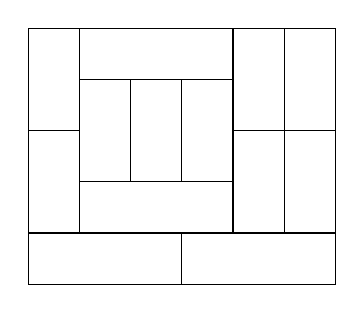
\begin{tikzpicture}[x=0.65cm,y=0.65cm]
				\draw (0,0) to (6,0) to (6,5) to (0,5) to cycle;
				\draw (0,1) to (3,1) to (3,0);
				\draw (3,1) to (6,1);
				\draw (0,3) to (1,3);
				\draw (1,1) to (1,5);
				\draw (4,3) to (6,3);
				\draw (4,1) to (4,5);
				\draw (5,1) to (5,5);
				\draw (1,2) to (4,2);
				\draw (1,4) to (4,4);
				\draw (2,2) to (2,4);
				\draw (3,2) to (3,4);
			\end{tikzpicture} & & 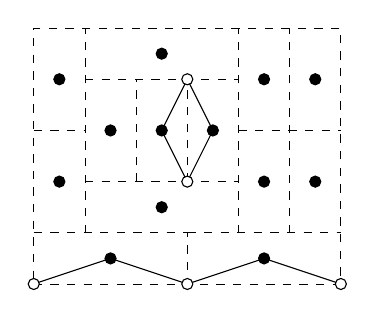
\begin{tikzpicture}[x=0.65cm,y=0.65cm]
				\begin{scope}[line width=0.3,dashed]
					\draw (0,0) to (6,0) to (6,5) to (0,5) to cycle;
					\draw (0,1) to (3,1) to (3,0);
					\draw (3,1) to (6,1);
					\draw (0,3) to (1,3);
					\draw (1,1) to (1,5);
					\draw (4,3) to (6,3);
					\draw (4,1) to (4,5);
					\draw (5,1) to (5,5);
					\draw (1,2) to (4,2);
					\draw (1,4) to (4,4);
					\draw (2,2) to (2,4);
					\draw (3,2) to (3,4);
				\end{scope}
				\coordinate (A) at (0,0);
				\coordinate (B) at (6,0);
				\coordinate (E) at (0.5,2);
				\coordinate (F) at (0.5,4);
				\coordinate (G) at (1.5,0.5);
				\coordinate (H) at (4.5,0.5);
				\coordinate (I) at (2.5,1.5);
				\coordinate (J) at (4.5,2);
				\coordinate (K) at (4.5,4);
				\coordinate (L) at (5.5,2);
				\coordinate (M) at (5.5,4);
				\coordinate (N) at (1.5,3);
				\coordinate (O) at (2.5,3);
				\coordinate (P) at (3.5,3);
				\coordinate (Q) at (2.5,4.5);
				\coordinate (R) at (3,0);
				\coordinate (S) at (3,2);
				\coordinate (T) at (3,4);
				\draw (A) to (G) to (R) to (H) to (B);
				\draw (O) to (S) to (P) to (T) to cycle;
				\draw[fill=white] (A) circle (2pt);
				\draw[fill=white] (B) circle (2pt);
				\draw[fill=black] (E) circle (2pt);
				\draw[fill=black] (F) circle (2pt);
				\draw[fill=black] (G) circle (2pt);
				\draw[fill=black] (H) circle (2pt);
				\draw[fill=black] (I) circle (2pt);
				\draw[fill=black] (J) circle (2pt);
				\draw[fill=black] (K) circle (2pt);
				\draw[fill=black] (L) circle (2pt);
				\draw[fill=black] (M) circle (2pt);
				\draw[fill=black] (N) circle (2pt);
				\draw[fill=black] (O) circle (2pt);
				\draw[fill=black] (P) circle (2pt);
				\draw[fill=black] (Q) circle (2pt);
				\draw[fill=white] (R) circle (2pt);
				\draw[fill=white] (S) circle (2pt);
				\draw[fill=white] (T) circle (2pt);
			\end{tikzpicture} &
		\end{tabularx}
	\end{figure}	
	Nun betrachten wir die Grade der Knoten in $G$. Wenn $v$ der Mittelpunkt eines kleinen Rechtecks $R$ ist, dann ist $d(v)$ gerade. Denn wenn $R$ ein $a\times 1$-Rechteck ist, dann muss für jeden Eckpunkt, der in $G$ liegt, auch der Eckpunkt am anderen Ende der horizontalen Kante mit Länge $a$ in $G$ liegen. Wenn $R$ ein $1\times b$-Rechteck ist, muss analog der Eckpunkt am anderen Ende der vertikalen Kante mit Länge $b$ ebenfalls in $G$ liegen. Wenn $v\neq A,B,C,D$ der Eckpunkt eines Rechtecks ist, dann muss $v$ ebenfalls geraden Grad haben, denn $v$ ist stets Eckpunkt von zwei oder vier kleinen Rechtecken.
	
	Wir wissen aber, dass $G$ einen Knoten mit ungeradem Grad enthält, denn $A$ liegt in $G$ und hat Grad~1. Weil die Anzahl der Knoten ungeraden Grades stets gerade ist, muss es in $G$ mindestens einen weiteren Knoten $w$ mit ungeradem Grad geben. Nach den obigen Überlegungen muss $w$ einer der Eckpunkte $B$, $C$ oder $D$ sein. Dann muss die $x$-Koordinate eines der Eckpunkte $B$, $C$ oder $D$ durch $a$ und seine $y$-Koordinate durch $b$ teilbar sein. Daraus folgt aber genau, dass $m$ durch $a$ oder $n$ durch $b$ teilbar ist.
\end{proof}
